\chapter{Tiling Hubbard}
\section{The Philosophy of Auxiliary Models}

In the previous chapter, we extended the Anderson impurity model to host a correlation-driven delocalisation-localisation transition on the impurity site, from a local Fermi liquid state to a local moment state.
We demonstrated that this transition captures very well the phenomenology of the Hubbard dimension in infinite dimensions (as seen from, say, dynamical mean-field theory (DMFT)).
In this chapter, we extend this approach by developing a formalism to study the more realistic case of finite-dimensional interacting models by using appropriately chosen impurity models as auxiliary models.
The key to an {\it auxiliary model method} is to construct an appropriate auxiliary model that while being tractable captures some essential property of the full lattice model~\cite{martin_2016}.
This involves separating the complete degrees of freedom into a system part (\(H_S\)) which one treats exactly and the rest of the system (\(H_R\)) that one might simplify in order to be able to solve the problem.
The non-trivial nature of the problem arises of course from the hybridisation \(H_{SR}\) between the system and the bath:
\begin{equation}\begin{aligned}
	{H} &= \begin{bmatrix} & {H}_{R} && {H}_{RS} & \\ & {H}_{RS}^* && {H}_{S} & \end{bmatrix}~.
\end{aligned}\end{equation}

This separation can always be done exactly, if one does not care about tractability. For example, one can take the Hubbard model that describes electrons hopping on a lattice and interacting when two electrons reside on the same lattice site:
\begin{equation}\begin{aligned}
	H_\text{hub} = -t\sum_{\langle i,j \rangle,\sigma }(c^\dagger_{i,\sigma}c_{j,\sigma} + \text{h.c.}) + U\sum_{i}n_{i \uparrow}n_{i \downarrow}~,
\end{aligned}\end{equation}
and separate this into parts, the system being the local orbitals of a specific site \(l\) and the rest of the system being all the other sites:
\begin{equation}\begin{aligned}
	H_S = U n_{l \uparrow} n_{l \downarrow},~~ H_R = -t\sum_{\langle i,j \rangle,\sigma }^\prime(c^\dagger_{i,\sigma}c_{j,\sigma} + \text{h.c.}) + U\sum_{i}^\prime n_{i \uparrow}n_{i \downarrow},~~ H_{SR} + H_{RS} = -t\sum_{i,\sigma} (c^\dagger_{l,\sigma}c_{i,\sigma} + \text{h.c.})~,
\end{aligned}\end{equation}
where the primed summation is carried out over all nearest-neighbour pairs that do not involve \(l\) and the summation in \(H_{SR} + H_{RS}\) is over all sites adjacent to \(l\).

The smaller system \(H_S\) (often called the {\it cluster}) is typically chosen such that its eigenstates are known exactly. Progress is then made by choosing a simpler form for \(H_R\) and its coupling \(H_{RS}\) with the smaller system. This combination of the cluster and the simpler bath is then called the \textit{auxiliary system}.
A tractable auxiliary system for the Hubbard model is the single-impurity Anderson model (SIAM); the correlated impurity site represents the set of local orbitals of any given site, while the conduction bath represents the rest of the lattice sites in an approximate fashion.  Such a construction is shown in fig.~\ref{cluster-bath}.
\begin{figure}[!htb]
	\centering
    \includegraphics[width=0.9\textwidth]{clusterBath.pdf}
	\caption{\textit{Left}: Full Hubbard model lattice with onsite repulsion $U^H$ on all sites and hopping between nearest neighbour sites with strength $t^H$. \textit{Right}: Extraction of the auxiliary (cluster+bath) system from the full lattice. The central site on left becomes the impurity site (red) on the right (with an onsite repulsion $\epsilon_d$), while the rest of the $N-1$ sites on the left form a conduction bath (green circles) (with dispersion $\epsilon_k$ and correlation modelled by the self-energy $\Sigma_k(\omega)$) that hybridizes with the impurity through the coupling $V$.}
	\label{cluster-bath}
\end{figure}

It should be noted that any reasonable choice of the cluster and bath would break the translational symmetry of the full model: To allow computing quantities, one would need to make the bath (which is a much larger system) simpler than the cluster (which is a single site). This distinction breaks the translational symmetry of the Hubbard model. As a result, calculations that make use of the translation symmetry of the full model (such as \(k-\)space objects) will require a periodisation operation of an auxiliary model quantity.

The present work is aimed towards developing a new auxiliary model method to study correlated electronic systems. As described above, the first step is to identify the correct impurity model which can faithfully capture the physics of the lattice model we are trying to solve. The local behaviour of this impurity model should reflect the essential local physics of the lattice model. Typically, we will consider impurity model geometries where the real-space bath site connected directly to the impurity hosts some local interaction. We will henceforth refer to this site as the {\it zeroth site}. This model must be solved using an impurity solver. In the present work, we use the recently-developed unitary renormalisation group method~\cite{anirbanmott1,anirbanmott2,anirbanurg1,anirbanurg2,siddharthacpi,santanukagome}. The leap to the bulk model is then made by applying {\bf manybody lattice translation operators} on the auxiliary model. This process, referred to as {\it tiling} here, allows us to reconstruct the lattice model Hamiltonian from that of the auxiliary model and restores the translation invariance of the full lattice model. Once the Hamiltonians can be mapped onto one another, it is possible to relate the eigenstates and correlations functions between the auxiliary model and lattice model, using a manybody version of {\bf Bloch's theorem}. 

\section{What Is The Correct Auxiliary Model For Correlated Electrons on a 2D Square Lattice?}\label{identifyModel}
As discussed in more detail in the previous chapter, it was necessary to extend the single-impurity Anderson model (SIAM) in order to obtain a phase transition on the impurity site. Without any modification, the standard Anderson model (at particle-hole symmetry) leads to the emergence of an \(\omega=0\) Kondo resonance in the impurity (\(d\sigma\)) spectral function at any value of the impurity correlation \(U_d\), at sufficiently low temperatures:
\begin{equation}\begin{aligned}
	H_\text{SIAM} = \sum_{k,\sigma}\varepsilon_k n_{k,\sigma} - V\sum_{\sigma}(c^\dagger_{0,\sigma}c_{d,\sigma} + \text{h.c.}) + \varepsilon_d \sum_\sigma n_{d,\sigma} + U_dn_{d, \uparrow}n_{d,\downarrow}~.
\end{aligned}\end{equation}
The operator \(c_{0,\sigma}\) acts on the local conduction bath density that couples with the impurity site. The low-energy is one of local Fermi liquid for all parameter regimes. Increasing \(U_d\) only serves to reduce the width of the central peak at the cost of the appearance of side bands at energy scales of the order of \(U_d\), but the resonance never disappears. The extended Anderson model that we developed augments the SIAM by allowing for local correlation in the local conduction bath charge density that couples with the impurity spin:
\begin{equation}\begin{aligned}\label{eSIAM}
	H_\text{ESIAM} = H_\text{SIAM} + J_K {\bm S}_d \cdot {\bm S}_0 - \frac{U_b}{2}\left(n_{0, \uparrow}^2 - n_{0, \downarrow}^2\right);
\end{aligned}\end{equation}
tuning this bath correlation to large attractive values (see~\cite{gazizovaleblanc2023} for some recent findings of non-local effective attractive interactions within the Hubbard model) {\it does} lead to a localisation transition on the impurity where the local Fermi liquid excitations are replaced by the physics of a gapped local moment on the impurity.
We note that the generation of such correlations in the bath is something that occurs in DMFT as well -- the conduction bath acquires a {\it non-trivial self-energy} during the convergence to self-consistency.

While this modified impurity model captures well the Mott metal-insulator transition of the Hubbard model in infinite dimensions, it {\it lacks any knowledge of the underlying lattice geometry}, and is therefore ill-suited to address the phenomenology of more realistic low-dimensional models. Examples of such phenomenology include the pseudogap phase of the cuprates (with nodal-antinodal dichotomy), strange metal (with \(T-\)linear resistivity) and high-\(T_c\) superconducting phases observed in several families of quantum materials as well as graphene. This leads us to propose the framework of {\it lattice-embedded quantum impurity models}. Upon embedding the impurity site within the underlying lattice, the coupling between it and its environment must be consistent with the lowered symmetry of the lattice (see Fig.~\ref{embedding}). Impurity-bath correlations calculated within such an impurity model are sensitive to the lattice geometry, and are much better suited to address the phenomenology mentioned above.

\begin{figure}[!htpb]
	\centering
	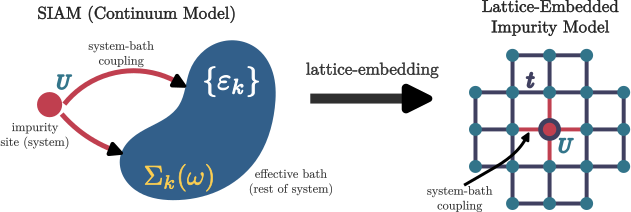
\includegraphics[width=1\textwidth]{embedding.pdf}
	\caption{}
	\label{embedding}
\end{figure}

As a concrete example, we take the extended SIAM defined in eq.~\ref{eSIAM}, and write down its lattice-embedded form on a 2D square lattice, with the impurity placed at the site \(r_d\). This is done by allowing the impurity to hybridise with the four nearest-neighbours, through \(V\) and \(J_K\). The same four sites also carry the local bath interaction. The complete auxiliary model is
\begin{equation}\begin{aligned}\label{LE-ESIAM}
	H =& -t\sum_{\langle i,j \rangle ,\sigma}(c^\dagger_{i, \sigma}c_{j,\sigma} + \text{h.c.}) + \sum_{\langle i, r_d \rangle}\left[-\frac{V}{Z}\sum_{\sigma }(c^\dagger_{r_d,\sigma}c_{i,\sigma} + \text{h.c.}) + \frac{J_K}{Z} {\bm S}_{r_d} \cdot {\bm S}_i - \frac{W}{2Z}\left(n_{i, \uparrow}^2 - n_{i, \downarrow}^2\right)\right]\\
	   & + \varepsilon_d \sum_\sigma n_{\bm r_d,\sigma} + U_d n_{\bm r_d, \uparrow} n_{\bm r_d,\downarrow},
\end{aligned}\end{equation}
where \(Z\) is the coordination number of the lattice, and the second summation \(\sum_{\langle i, r_d \rangle}\) is carried out over all sites \(i\) that are nearest-neighbour to the site \(r_d\). Note that the one-particle hybridisation \(V\) and the spin-exchange coupling \(J_K\) have their {\it symmetry lowered} from the \(s-\)wave spherical symmetry of the continuum impurity models to a \(C_4\)-symmetry consistent with the underlying lattice. This feature is crucial in explaining the phenomenology of the various low-dimensional materials.

Various enhancements can be applied to such a model. The lattice can be modified to study different materials. More complicated geometries such as a two-layer model can be studied using a two-impurity auxiliary model, where each impurity couples with it's own conduction bath as well as to each other.

\section{Mapping Auxiliary Model To Lattice Model: Tiling Formalism}
In this subsection, we provide an explicit example of constructing a lattice model from a lattice-embedded impurity model. This will involve the use of manybody lattice translation operators, so we begin with a brief discussion of them.

\subsection{Manybody Translation Operators}\label{translationOperators}

In order to create the bulk model, we need to translate the local auxiliary model over the entire lattice. For this, we define {\it many-particle global} translation operators \(T({\bm a})\) that translate all positions by a vector \({\bm a}\). In terms of manybody states and operators, their action is defined as 
\begin{equation}\begin{aligned}\label{translationDefinition}
	&T^\dagger({\bm a}) \ket{{\bm r}_1, {\bm r}_2,\ldots} = \ket{{\bm r}_1 + {\bm a}}\otimes\ket{{\bm r}_2 + {\bm a}}\ldots\otimes\ket{{\bm r}_n + {\bm a}}\\
	&T^\dagger({\bm a}) \mathcal{O}\left({\bm r}_1, {\bm r}_2,\ldots\right)T({\bm a}) = \mathcal{O}\left({\bm r}_1 + {\bm a}, {\bm r}_2 + {\bm a},\ldots\right)~,
\end{aligned}\end{equation}
where \(\ket{{\bm r}_1, {\bm r}_2,\ldots}\) is a state in the manyparticle Fock-space basis with the particles localised at the specified positions. For example, for a local fermionic creation operator \(c^\dagger({\bm r})\), we have 
\begin{equation}\begin{aligned}
	T^\dagger({\bm a}) c^\dagger({\bm r}) T({\bm a}) = c^\dagger({\bm r} + {\bm a})~.
\end{aligned}\end{equation}
It acts similarly on the auxiliary model Hamiltonian:
\begin{equation}\begin{aligned}
	T^\dagger({\bm a}){H}_\text{aux}({\bm r}_d)T({\bm a}) = {H}_\text{aux}({\bm r}_d + {\bm a})~,
\end{aligned}\end{equation}
translating all sites by the vector \({\bm a}\). By introducing the Fourier transform to momentum space,
\begin{equation}\begin{aligned}
	\ket{{\bm r}_1, {\bm r}_2,\ldots} = \otimes_{j=1}^N \int d{\bm k}_j e^{i {\bm r}_j\cdot{\bm k}_j} \ket{{\bm k}_j}~,
\end{aligned}\end{equation}
it is easy to see that the total momentum states are eigenstates of the global translation operators:
\begin{equation}\begin{aligned}
	T^\dagger({\bm a})\ket{{\bm k}_1, {\bm k}_2,\ldots} &= \otimes_{j=1}^N \int d{\bm r}_j e^{-i {\bm r}_j\cdot{\bm k}_j} T^\dagger({\bm a})\ket{{\bm r}_j}~,\\
							    &=\otimes_{j=1}^N \int d{\bm r}_j e^{-i {\bm r}_j\cdot{\bm k}_j} \ket{{\bm r}_j + {\bm a}}\\
							    &=\otimes_{j=1}^N e^{i {\bm a}\cdot{\bm k}_j}\int d{\bm r}_j e^{-i {\bm r}_j\cdot{\bm k}_j} \ket{{\bm r}_j}\\
							    &=e^{i {\bm a}\cdot{\bm k}_\text{tot}}\ket{{\bm k}_1, {\bm k}_2,\ldots},
\end{aligned}\end{equation}
where \({\bm k}_\text{tot} = \sum_j {\bm k}_j\) is the total momentum. This gives a compact form for the translation operator:
\begin{equation}\begin{aligned}
	T^\dagger({\bm a}) = e^{i {\bm a}\cdot{\bm{\hat k}}_\text{tot}}~,
\end{aligned}\end{equation}
where \(\hat {\bm k}_\text{tot}\) is the total momentum operator.

We end this section by calculating the effect of the translation operators on the \(k-\)space annihilation operators. We have
\begin{equation}\begin{aligned}\label{fourTransf}
	c({\bm k}) = \frac{1}{\sqrt N}\sum_{\bm r}e^{-i{\bm k}\cdot{\bm r}}c({\bm r})~.
\end{aligned}\end{equation}
Applying the translation operator to this decomposition, we get
\begin{equation}\begin{aligned}\label{translationOnField}
	T\left(\vec a\right) c({\bm k}) T^\dagger\left(\vec a\right) &= \frac{1}{\sqrt N}\sum_{\bm r}e^{-i{\bm k}\cdot{\bm r}}T\left(\vec a\right) c({\bm r}) T^\dagger\left(\vec a\right) \\
																 &= \frac{1}{\sqrt N}\sum_{\bm r}e^{-i{\bm k}\cdot{\bm r}}c({\bm r} - \vec a) \\
																 &= e^{-i{\bm k}\cdot\vec a}c({\bm k})~.
\end{aligned}\end{equation}

\subsection{Periodisation of Auxiliary Model Into Extended Hubbard Model}\label{hamiltonianTile}
We recall the lattice-embedded impurity model defined in eq.~\ref{LE-ESIAM}.
As discussed above, the route to restoring translation symmetry and reconstructing the lattice model is to translate the auxiliary model using manybody translation operators.
Accordingly, we identify the ``unit cell'' of translation.
Since we expect the impurity site to capture most of the physics arising from the correlated electrons, a good choice for the unit cell is the impurity site and it's surrounding correlated environment. In order to retain information of the lattice geometry, we convert the hybridisation and bath interaction terms from real space to \(k-\)space. The Hamiltonian for the unit cell is therefore
\begin{equation}\begin{aligned}\label{clusterHamiltonian}
	H_\text{clust}(\bm r_d) =& -\sum_{{\bm k},\sigma} e^{i \bm k \cdot \bm r_d } V({\bm k})(c^\dagger_{{\bm r}_d,\sigma} c_{{\bm k},\sigma} + \text{h.c.}) + \sum_{\bm k_1, \bm k_2} e^{i (\bm k_1 - \bm k_2) \cdot \bm r_d }~J_K({\bm k_1, \bm k_2}) {\bm S}_{\bm r_d} \cdot {\bm S}_{\bm k_1, \bm k_2} + \varepsilon_d n_{\bm r_d}\\
							 & + U_d n_{{\bm r_d}, \uparrow} n_{{\bm r_d}, \downarrow}- \frac{1}{2}\sum_{\{\bm k_i\},\sigma,\sigma^\prime}\sigma~\sigma^\prime~e^{i (\bm k_1 - \bm k_2 + \bm k_3 - \bm k_4) \cdot \bm r_d } W(\{\bm k_i\}) c^\dagger_{\bm k_1, \sigma}c_{\bm k_2, \sigma}c^\dagger_{\bm k_3, \sigma^\prime}c_{\bm k_4, \sigma^\prime}~,
\end{aligned}\end{equation}
where \({\bm S}_{\bm k_1, \bm k_2} = \sum_{\alpha,\beta}{\bm \sigma}_{\alpha,\beta} c^\dagger_{\bm k_1,\alpha}c_{\bm k_2,\beta}\), and the Fourier transforms are defined by the following relations:
\begin{equation}\begin{aligned}\label{FTauxiliary}
	\sum_{{\bm k}} e^{i \bm k \cdot \bm r_d } V({\bm k})c^\dagger_{{\bm r}_d,\sigma} c_{{\bm k},\sigma} &= \frac{V}{Z}\sum_{r \to \text{NN of }\bm r_d} c^\dagger_{{\bm r}_d,\sigma}c_{{\bm r},\sigma}~,\\
	\sum_{\bm k_1, \bm k_2} e^{i (\bm k_1 - \bm k_2) \cdot \bm r_d }~J_K({\bm k_1, \bm k_2}) \vec{S}_{\bm r_d} \cdot \vec{S}_{\bm k_1, \bm k_2} &= \frac{J_K}{Z}\sum_{r \to \text{NN of }\bm r_d} {\bm S}_{\bm r_d} \cdot {\bm S}_{\bm r}~,\\
	\sum_{\bm k_1, \bm k_2, \bm q_1, \bm q_2}e^{i (\bm k_1 - \bm k_2 + \bm k_3 - \bm k_4) \cdot \bm r_d } W(\{\bm k_i\}) c^\dagger_{\bm k_1, \sigma}c_{\bm k_2, \sigma}c^\dagger_{\bm k_3, \sigma^\prime}c_{\bm k_4, \sigma^\prime} &= \frac{W}{2Z}\sum_{r \to \text{NN of }\bm r_d} n_{\bm r, \sigma}n_{\bm r, \sigma^\prime}~,
\end{aligned}\end{equation}


We now translate this unit cell to all sites of the lattice, and reconstruct a translationally-invariant correlated lattice model:
\begin{equation}\begin{aligned}\label{tilingPrescription}
	{H}_\text{latt} = \sum_{{\bm r}}T^\dagger({\bm r} - {\bm r}_d)H_\text{clust}(\bm r_d)T({\bm r} - {\bm r}_d)~.
\end{aligned}\end{equation}
We consider the effect of the translation operations on each part of the Hamiltonian. The purely local terms translate directly into a chemical potential term and a Hubbard interaction term:
\begin{equation}\begin{aligned}
	\sum_{{\bm r}}T^\dagger({\bm r} - {\bm r}_d) (\varepsilon_d \sum_\sigma n_{\bm r_d,\sigma} + U_d n_{{\bm r_d}, \uparrow} n_{{\bm r_d}, \downarrow})T({\bm r} - {\bm r}_d) = \varepsilon_d \sum_{\bm r, \sigma} n_{\bm r,\sigma} + U_d \sum_{\bm r}n_{{\bm r}, \uparrow} n_{{\bm r}, \downarrow}~.
\end{aligned}\end{equation}
The one-particle hybridisation term maps onto a tight-binding hopping term:
\begin{equation}\begin{aligned}
	\sum_{{\bm r}}T^\dagger({\bm r} - {\bm r}_d) \sum_{\bm k} e^{i \bm k \cdot \bm r_d }V(\bm k)c^\dagger_{{\bm r}_d,\sigma} c_{{\bm k},\sigma}T({\bm r} - {\bm r}_d) &= \sum_{{\bm r}}\sum_{\bm k} e^{i \bm k \cdot \bm r} V(\bm k) c^\dagger_{{\bm r},\sigma} c_{{\bm k},\sigma}\\
																																									  &= \frac{V}{Z}\sum_{\bm r}\sum_{\bm r^\prime \to \text{NN of~}\bm r}  c^\dagger_{{\bm r},\sigma} c_{{\bm r}^\prime,\sigma}\\
																																									  &= \frac{2V}{Z}\sum_{\langle \bm r,\bm r^\prime \rangle}  c^\dagger_{{\bm r},\sigma} c_{{\bm r}^\prime,\sigma}~,
\end{aligned}\end{equation}
where we used eq.~\ref{translationOnField} and the first equation from~\ref{FTauxiliary}, and the fact that each nearest-neighbour pair \(\bm r, \bm r^\prime\) appears twice in the summation.

The Kondo terms map onto a nearest-neighbour spin-exchange term:
\begin{equation}\begin{aligned}
	\sum_{\bm r,\bm k_1, \bm k_2}T^\dagger({\bm r} - {\bm r}_d) e^{i (\bm k_1 - \bm k_2) \cdot \bm r_d }~J_K({\bm k_1, \bm k_2}) \vec{S}_{\bm r_d} \cdot \vec{S}_{\bm k_1, \bm k_2} T({\bm r} - {\bm r}_d) &= \sum_{\bm r,\bm k_1, \bm k_2} e^{i (\bm k_1 - \bm k_2) \cdot \bm r }~J_K({\bm k_1, \bm k_2}) \vec{S}_{\bm r} \cdot \vec{S}_{\bm k_1, \bm k_2} \\
																																																		 &=\frac{J_K}{Z}\sum_{\bm r}\sum_{\bm r^\prime \to \text{NN of~}\bm r} \vec{S}_{\bm r} \cdot \vec{S}_{\bm r^\prime}~,\\
																																																		 &=\frac{2J_K}{Z}\sum_{\langle \bm r,\bm r^\prime \rangle } \vec{S}_{\bm r} \cdot \vec{S}_{\bm r^\prime}~,
\end{aligned}\end{equation}
where we used the second equation from~\ref{FTauxiliary}. Finally, the bath interaction term \(W\) maps onto another Hubbard term
\begin{equation}\begin{aligned}
	&\sum_{\bm r,\bm k_1, \bm k_2, \bm k_3, \bm k_4}T^\dagger({\bm r} - {\bm r}_d) e^{i (\bm k_1 - \bm k_2 + \bm k_3 - \bm k_4) \cdot \bm r_d } W(\{\bm k_i\}) c^\dagger_{\bm k_1, \sigma}c_{\bm k_2, \sigma}c^\dagger_{\bm k_3, \sigma^\prime}c_{\bm k_4, \sigma^\prime} T({\bm r} - {\bm r}_d) \\
	&= \sum_{\bm r,\bm k_1, \bm k_2, \bm k_3, \bm k_4}e^{i (\bm k_1 - \bm k_2 + \bm k_3 - \bm k_4) \cdot \bm r } W(\{\bm k_i\}) c^\dagger_{\bm k_1, \sigma}c_{\bm k_2, \sigma}c^\dagger_{\bm k_3, \sigma^\prime}c_{\bm k_4, \sigma^\prime} \\
	&= \frac{W}{2Z}\sum_{\bm r}\sum_{\bm r^\prime \to \text{NN of}~\bm r}n_{\bm r^\prime,\sigma}n_{\bm r^\prime,\sigma^\prime}\\
	&= \frac{W}{2}\sum_{\bm r}n_{\bm r,\sigma}n_{\bm r,\sigma^\prime}~,
\end{aligned}\end{equation}
where we used the fact that each point \(\bm r^\prime\) (which we relabel as \(r\)) appears \(Z\) times in the summation.

The complete lattice Hamiltonian, after applying the translation operators, is
\begin{equation}\begin{aligned}
	H_\text{latt} = \varepsilon_d \sum_{\bm r, \sigma} n_{\bm r,\sigma} + U_d \sum_{\bm r}n_{{\bm r}, \uparrow} n_{{\bm r}, \downarrow} - \frac{2V}{Z}\sum_{\langle \bm r,\bm r^\prime \rangle}  c^\dagger_{{\bm r},\sigma} c_{{\bm r}^\prime,\sigma} + \frac{2J_K}{Z}\sum_{\langle \bm r,\bm r^\prime \rangle } \vec{S}_{\bm r} \cdot \vec{S}_{\bm r^\prime} - \frac{W}{2}\sum_{\bm r}\left(n_{\bm r,\uparrow} - n_{\bm r, \downarrow}\right)^2~.
\end{aligned}\end{equation}
This is clearly an extended Hubbard model, with both 1-particle and spin-exchange nearest-neighbour hybridisation. The general form of the model is
\begin{equation}\begin{aligned}
	H_\text{ex-Hub} = -t\sum_{\langle i,j \rangle,\sigma}(c^\dagger_{i,\sigma}c_{j,\sigma} + \text{h.c.}) + J\sum_{\langle i,j \rangle}{\bm S}_i \cdot {\bm S}_j + U\sum_i n_{i,\uparrow} n_{i, \downarrow} - \mu \sum_{i,\sigma}n_{i,\sigma}~,
\end{aligned}\end{equation}
such that the effective couplings resulting from the tiling operation is
\begin{equation}\begin{aligned}
t = \frac{2V}{Z}, ~J = \frac{2J_K}{Z},~U=U_d - W,~\mu = -\varepsilon_d + \frac{W}{2}~.
\end{aligned}\end{equation}

\subsection{Form Of The Eigenstates: Bloch's Theorem}
The tiled Hamiltonian defined in eq.~\ref{tilingPrescription} is manifestly symmetric under discrete translation, given that it's expressed in terms of the translation operators. The fact that the Hamiltonian \(H_\text{latt}\) commutes with the manybody translation operator implies that the total crystal momentum is a conserved quantity. We will now use this to write down a ``tiling" relation between the eigenstates of the auxiliary model and those of the lattice model.

In the tight-binding approach to lattice problems, the full Hamiltonian is obtained by translating the dynamics of the localised orbitals at each site over the entire lattice. The full eigenstate \(\ket{\Psi}\) is obtained by constructing liner combinations of the eigenstates \(\ket{\psi(i)}\) of the local Hamiltonians. According to Bloch's theorem, \(\ket{\Psi}\) is of the form \(\ket{\Psi_{n,\bm K}} = \sum_{i} e^{i {\bm K}\cdot{\bm r}_i} \ket{\psi_n(i)}\), where \({\bm K}\) is the single-particle crystal momentum, \(n\) is the band-index that labels various states within the local orbital, and \({\bm r}_i\) sums over the positions of the local Hamiltonians. Bloch's theorem ensures that eigenstates satisfy the following relation under a translation operation by an arbitrary number of lattice spacings \({n\bm a}\):
\begin{equation}\begin{aligned}
	T^\dagger(l{\bm a})\ket{\Psi_{n,{\bm K}}} = \sum_{i} e^{i {\bm K}\cdot{\bm r}_i} \ket{\psi_n(i + l)} = e^{-il{\bm K}\cdot{\bm a}}\ket{\Psi_{n,\bm K}}~.
\end{aligned}\end{equation}
% The definition and some properties of these global translation operations were provided in Appendix~\ref{translationOperators}. It was shown there that they share eigenstates with the total momentum operator. In a lattice model, this continuous symmetry gets lowered to its discrete form: the total {\it crystal} momentum is conserved by any scattering process. As a result, the eigenstates can be labelled using the combined index \(s = \left({\bm k}, n\right) \) where \({\bm k}\) is the total crystal momentum and \(n\) is a band index \(n\).

As discussed earlier, the eigenstates \(\ket{\Psi_{n,\bm K}}\) of the lattice Hamiltonian obtained using eq.~\ref{tilingPrescription} enjoy the discrete translation symmetry of the lattice, and therefore enjoy a {\it many-body} Bloch's theorem~\cite{stoyanova}. This means that the {\it local} eigenstates \(\ket{\psi_n\left({\bm r}_d\right)}\) (with the impurity located at an arbitrary position \({\bm r}_d\)) of the unit cell auxiliary model Hamiltonian \({H}_\text{clust}({\bm r}_d)\) defined in eq.~\ref{clusterHamiltonian} can be used to construct eigenstates of the lattice Hamiltonian. The index \(n(=0,1,\ldots)\) in the subscript indicates that it is the \(n^\text{th}\) eigenstate of the auxiliary model. The following combination of the auxiliary model eigenstates satisfies a many-particle equivalent of Bloch's theorem~\cite{stoyanova}:
\begin{equation}\begin{aligned}\label{eigenstateProposal}
	\ket{\Psi_{s}} \equiv \ket{\Psi_{{\bm K}, n}} &= \frac{1}{\sqrt N}\sum_{{\bm r}_d} e^{i {\bm K}\cdot{\bm r}_d} \ket{\psi_{n}\left({\bm r}_d\right)}~,
\end{aligned}\end{equation}
where \(N\) is the total number of lattice sites and \({\bm r}_d\) is summed over all lattice spacings. The set of \(n=0\) states form the lowest band in the spectrum of the lattice, while higher values of \(n\) produce the more energetic bands.

\section{Mapping Greens Functions from Auxiliary Model to Lattice Model}\label{tilingGreensFunction}
\subsection{One-particle \(k-\)space Greens functions}\label{tileKspaceGreen}
In the previous part, we proposed a form for the eigenstates \(\ket{\Psi_s}\) of the bulk Hamiltonian in terms of the ground-states \(\ket{\psi_n}\) of the auxiliary models.
In this section, we will relate one-particle Greens functions of the lattice model to those of the auxiliary model. We define the retarded time-domain lattice \(k-\)space Greens function at zero temperature as
\begin{equation}\begin{aligned}
	G({\bm k}\sigma; t) = -i\theta(t) \braket{\Psi_\text{gs} | \{ c_{{\bm k}\sigma}(t), c^\dagger_{{\bm k}\sigma} \} | \Psi_\text{gs}}~.
\end{aligned}\end{equation}
where \(\ket{\Psi_\text{gs}}\) is the lattice groundstate. Time evolution of the operators is governed by the lattice Hamiltonian \(H_\text{latt}\):
\begin{equation}\begin{aligned}\label{heisenberg}
	c_{{\bm k}\sigma}(t) = e^{it H_\text{latt} }c_{{\bm k}\sigma}e^{-i t H_\text{latt}}~.
\end{aligned}\end{equation}
By using eq.~\ref{translationOnField} and the fact that the translation operators commute with \(H_\text{latt}\), we have the relation
\begin{equation}\begin{aligned}
	T\left(\vec a\right) c({\bm k})(t) T^\dagger\left(\vec a\right) = e^{-i{\bm k}\cdot\vec a}c({\bm k})(t)~,
\end{aligned}\end{equation}
which combined with eq.~\ref{translationOnField} gives
\begin{equation}\begin{aligned}\label{translationOnProduct}
	T\left(\bm a\right) c({\bm k})(t) c^\dagger({\bm k}) T^\dagger\left(\bm b\right) = e^{i{\bm k}\cdot(\bm b - \bm a)}c({\bm k})(t) T^\dagger({\bm b - \bm a}) c^\dagger({\bm k})~.
\end{aligned}\end{equation}



In order to make use of the mapping between auxiliary model and lattice model Hamiltonians, we would like to express this lattice Greens function in terms of auxiliary model Greens functions -- objects that can be computed purely from within a single auxiliary model. This will be a major simplification in our computations, because it is easier to work with a quantum impurity model, as compared to an interacting lattice model.

To make progress towards this, we express the lattice groundstate in terms of the auxiliary model groundstates (using eq.~\ref{eigenstateProposal}):
\begin{equation}\begin{aligned}\label{retarded}
	G({\bm k}\sigma; t) = -i\theta(t) \frac{1}{N}\sum_{\bm r_1,\bm r_2} \braket{\psi_\text{gs}({\bm r_2}) | \{ c_{{\bm k}\sigma}(t), c^\dagger_{{\bm k}\sigma} \} | \psi_\text{gs}({\bm r_1})}~.
\end{aligned}\end{equation}
We take one of the terms in the anticommutator and proceed to simplify it:
\begin{equation}\begin{aligned}
	\sum_{\bm r_1,\bm r_2} \braket{\psi_\text{gs}({\bm r_2}) | c_{{\bm k}\sigma}(t) c^\dagger_{{\bm k}\sigma} | \psi_\text{gs}({\bm r_1})} &= \sum_{\bm r_1,\bm r_2} \braket{\psi_\text{gs}({\bm r_d}) | T({\bm r_2 - \bm r_d}) c_{{\bm k}\sigma}(t) c^\dagger_{{\bm k}\sigma} T^\dagger({\bm r_1 - \bm r_d}) | \psi_\text{gs}({\bm r_d})}\\
																																		   &= \sum_{\bm r_1,\bm r_2} e^{i\bm k(\bm r_1 - \bm r_2)} \braket{\psi_\text{gs}({\bm r_d}) | c_{{\bm k}\sigma}(t) T^\dagger({\bm r_1 - \bm r_2}) c^\dagger_{{\bm k}\sigma} | \psi_\text{gs}({\bm r_d})}~\\
																																		   &= N\sum_{\bm r} e^{i\bm k \cdot\bm r} \braket{\psi_\text{gs}({\bm r_d}) | c_{{\bm k}\sigma}(t) T^\dagger(\bm r) c^\dagger_{{\bm k}\sigma} | \psi_\text{gs}({\bm r_d})}~.
\end{aligned}\end{equation}
where \({\bm r_d}\) is a reference lattice site, and we used eq.~\ref{translationOnProduct} in the second step. The other term in the anticommutator gives
\begin{equation}\begin{aligned}
	\sum_{\bm r_1,\bm r_2} \braket{\psi_\text{gs}({\bm r_2}) | c^\dagger_{{\bm k}\sigma} c_{{\bm k}\sigma}(t) | \psi_\text{gs}({\bm r_1})} &= \sum_{\bm r_1,\bm r_2} \braket{\psi_\text{gs}({\bm r_d}) | T({\bm r_2 - \bm r_d}) c^\dagger_{{\bm k}\sigma} c_{{\bm k}\sigma}(t) T^\dagger({\bm r_1 - \bm r_d}) | \psi_\text{gs}({\bm r_d})}\\
																																		   &= \sum_{\bm r_1,\bm r_2} e^{-i\bm k(\bm r_1 - \bm r_2)} \braket{\psi_\text{gs}({\bm r_d}) | c^\dagger_{{\bm k}\sigma} T^\dagger({\bm r_1 - \bm r_2}) c_{{\bm k}\sigma}(t) | \psi_\text{gs}({\bm r_d})}~\\
																																		   &= N\sum_{\bm r} e^{-i\bm k\cdot\bm r} \braket{\psi_\text{gs}({\bm r_d}) | c^\dagger_{{\bm k}\sigma} T^\dagger({\bm r}) c_{{\bm k}\sigma}(t) | \psi_\text{gs}({\bm r_d})}~.
\end{aligned}\end{equation}
To resolve the time evolution of the operators, we insert $1 = \sum_m \ket{\psi_m({\bm r_d})}\bra{\psi_m({\bm r_d})}$ into the equation. We again work with just the first term of the anticommutator for convenience:
\begin{equation}\begin{aligned}
	&\sum_{\bm r_1,\bm r_2} \braket{\psi_\text{gs}({\bm r_2}) | c_{{\bm k}\sigma}(t) c^\dagger_{{\bm k}\sigma} | \psi_\text{gs}({\bm r_1})} \\
	&= N\sum_{\bm r, n_1, n_2} e^{i\bm k \cdot\bm r} \braket{\psi_\text{gs}({\bm r_d}) | c_{{\bm k}\sigma}(t) \ket{\psi_{n_1}({\bm r_d})}\bra{\psi_{n_1}({\bm r_d})} T^\dagger(\bm r) \ket{\psi_{n_2}({\bm r_d})}\bra{\psi_{n_2}({\bm r_d})} c^\dagger_{{\bm k}\sigma} | \psi_\text{gs}({\bm r_d})}\\
	&= N\sum_{\bm r, n_1, n_2} e^{i\bm k \cdot\bm r} \braket{\psi_\text{gs}({\bm r_d}) | c_{{\bm k}\sigma}(t) \ket{\psi_{n_1}({\bm r_d})}\braket{\psi_{n_1}({\bm r_d}) | \psi_{n_2}({\bm r_d + \bm r})}\bra{\psi_{n_2}({\bm r_d})} c^\dagger_{{\bm k}\sigma} | \psi_\text{gs}({\bm r_d})}~.
\end{aligned}\end{equation}
The overlap \(\braket{\psi_{n_1}({\bm r_d}) | \psi_{n_2}({\bm r_d + \bm r})}\) between the eigenstates of the auxiliary models at \(\bm r_d\) and \(\bm r_d + \bm r\) are appreciable only for \(n_1 = n_2\). This is because, for small \(\bm r\), the auxiliary models are very similar and the states are therefore almost orthogonal. For large \(\bm r\), the overlap is again suppressed because the auxiliary model eigenstates are localised around the impurity. We therefore make the simplifying assumption: \(\braket{\psi_{n_1}({\bm r_d}) | \psi_{n_2}({\bm r_d + \bm r})} = \delta_{n_1, n_2}\braket{\psi_{n_1}({\bm r_d}) | \psi_{n_1}({\bm r_d + \bm r})} = \delta_{n_1, n_2}F_{n_1}(\bm r)\). Substituting this, we get
\begin{equation}\begin{aligned}\label{intermediate}
	\sum_{\bm r_1,\bm r_2} \braket{\psi_\text{gs}({\bm r_2}) | c_{{\bm k}\sigma}(t) c^\dagger_{{\bm k}\sigma} | \psi_\text{gs}({\bm r_1})} = N\sum_{n} F_n(\bm k) \braket{\psi_\text{gs}({\bm r_d}) | c_{{\bm k}\sigma}(t) \ket{\psi_{n}({\bm r_d})}\bra{\psi_{n}({\bm r_d})} c^\dagger_{{\bm k}\sigma} | \psi_\text{gs}({\bm r_d})}~,
\end{aligned}\end{equation}
where we have defined the Fourier transform \(F_n(\bm k) = \sum_{\bm r} e^{i\bm k \cdot\bm r} F_n(\bm r)\) of the overlap function.

We now consider more carefully the transition operator \(c_{{\bm k}\sigma}\) for the 1-particle excitation giving rise to the above Greens function. Within our auxiliary model approach, gapless excitations within the lattice model are represented by gapless excitations of the impurity site, specifically those that try to screen the impurity site. As a result, the uncoordinated scattering process \(c_{{\bm k}\sigma}\) for the lattice model must be replaced by a coherent excitation  \(\mathcal{T}\) within the impurity model that captures those gapless excitations that occur in connection with the impurity, and projects out the uncorrelated excitations that take place even when the impurity site is decoupled from the bath.

In order to construct this auxiliary model \(\mathcal{T}-\)matrix, we allow for all excitations of the impurity site in conjunction with those of the \(k-\)state:
\begin{equation}\begin{aligned}\label{tmatrix}
	\mathcal{T}_{{\bm k},\sigma} = \left[\left(\sum_{\sigma^\prime}c^\dagger_{\bm r_d\sigma} + \text{h.c.}\right) + \left(S_{\bm r_d}^+ + \text{h.c.}\right) + \left(C_{\bm r_d}^+ + \text{h.c.}\right)\right]c_{{\bm k}\sigma}~,
\end{aligned}\end{equation}
where \(S_{\bm r_d}^+\) and \(C_{\bm r_d}^+\) are spin and charge flip operators on the impurity site that cause transition from \(\ket{\downarrow} \to \ket{\uparrow}\) and \(\ket{0} \to \ket{\uparrow \downarrow}\) respectively.

Apart from modifying the excitation operator, we will now simplify the time-evolution as well. The first overlap on the right-hand side of eq.~\ref{intermediate} expands to
\begin{equation}\begin{aligned}
	\braket{\psi_\text{gs}({\bm r_d}) | \mathcal{T}_{{\bm k},\sigma}(t) | \psi_{n}({\bm r_d})} = \braket{\psi_\text{gs}({\bm r_d}) | e^{i(H_\text{aux}(\bm r_d) + H_\text{cav}(\bm r_d))t} \mathcal{T}_{{\bm k},\sigma} e^{-i(H_\text{aux}(\bm r_d) + H_\text{cav}(\bm r_d))t} | \psi_{n}({\bm r_d})}~,
\end{aligned}\end{equation}
where \(H_\text{aux}(\bm r_d)\) (eq.~\ref{LE-ESIAM}) is the auxiliary model Hamiltonian consisting of the cluster Hamiltonian \(H_\text{clust}(\bm r_d)\) along with all one-particle terms \(H_\text{1p}\) in the Hamiltonian (in a typical lattice model, this will be he tight-binding hopping terms), and \(H_\text{cav}(\bm r_d)\) is the ``cavity" Hamiltonian consisting of all interaction (2-particle and beyond) terms in the Hamiltonian. Together, they create the full lattice Hamiltonian: \(H_\text{latt} = H_\text{aux}(\bm r_d) + H_\text{cav}(\bm r_d)\). Using the Zassenhaus form of the Baker-Campbell-Hausdorff formula, we have
\begin{equation}\begin{aligned}
	e^{i(H_\text{aux}(\bm r_d) + H_\text{cav}(\bm r_d))t} \approx e^{iH_\text{aux}(\bm r_d)t} e^{i H_\text{cav}(\bm r_d)t}e^{[H_\text{aux}(\bm r_d),~H_\text{cav}(\bm r_d)]t^2/2}~,
\end{aligned}\end{equation}
where we have dropped the higher-order terms because the commutators involve only the boundary degrees of freedom and become subsequently smaller as the order increases. One can think of the operator \(e^{i H_\text{cav}(\bm r_d)t}e^{[H_\text{aux}(\bm r_d),~H_\text{cav}(\bm r_d)]t^2/2}\) as renormalising the auxiliary model \(\mathcal{T}-\)matrix through hybridisation with the rest of the system and formally leading to a new \(\mathcal{T}-\)matrix:
\begin{equation}\begin{aligned}
	\mathcal{T}_{{\bm k},\sigma}^* = e^{i H_\text{cav}(\bm r_d)t}e^{[H_\text{aux}(\bm r_d),~H_\text{cav}(\bm r_d)]t^2/2}\mathcal{T}_{{\bm k},\sigma}e^{-[H_\text{aux}(\bm r_d),~H_\text{cav}(\bm r_d)]t^2/2}e^{-i H_\text{cav}(\bm r_d)t}~.
\end{aligned}\end{equation}
One can also absorb the modulating phase factor \(F_n(\bm k)\) (defined above and appearing in eq.~\ref{intermediate}) into this renormalisation:
\begin{equation}\begin{aligned}
	\mathcal{T}_{{\bm k},\sigma}^* = e^{i H_\text{cav}(\bm r_d)t}e^{[H_\text{aux}(\bm r_d),~H_\text{cav}(\bm r_d)]t^2/2}\mathcal{T}_{{\bm k},\sigma}F_n(\bm k) \mathcal{P}_n({\bm r_d})~e^{-[H_\text{aux}(\bm r_d),~H_\text{cav}(\bm r_d)]t^2/2}e^{-i H_\text{cav}(\bm r_d)t}~,
\end{aligned}\end{equation}
where \(\mathcal{P}_n({\bm r_d})\) projects onto the \(n^\text{th}\) eigenstate \(\ket{\psi_{n}({\bm r_d})}\).

Since the overlap is calculated in the eigenstates of the auxiliary model at \(\bm r_d\), we adopt the zeroth order approximation of ignoring this renormalisation. Later, we will specify a prescription of systematically improving our computation. The overlap expression becomes
\begin{equation}\begin{aligned}
	\braket{\psi_\text{gs}({\bm r_d}) | \mathcal{T}_{{\bm k},\sigma}(t) | \psi_{n}({\bm r_d})} = \braket{\psi_\text{gs}({\bm r_d}) | e^{i(H_\text{clust}(\bm r_d) + H_\text{1p})t} \mathcal{T}_{{\bm k},\sigma} e^{-i(H_\text{clust}(\bm r_d) + H_\text{1p})t} | \psi_{n}({\bm r_d})}~.
\end{aligned}\end{equation}
To make the problem tractable, we treat the effect of \(H_\text{1p}\) at the level of an expectation value and note that the effect of the transition operator is to create a hole of momentum \(\bm k\) (eq.~\ref{tmatrix}). Let the Hamiltonian \(H_\text{1p}\) be diagonal in certain modes \(c_{\nu,\sigma}\) with energies \(\epsilon_\nu\), and the operator \(c_{\bm k,\sigma}\) can be expressed in terms of these modes: \(c_{\bm k,\sigma} = \sum_{\nu}C_{\nu,\bm k}c^\dagger_{\nu,\sigma}\). A similar decomposition will hold for the \(\mathcal{T}-\)matrix. Substituting it gives
\begin{equation}\begin{aligned}
	\braket{\psi_\text{gs}({\bm r_d}) | \mathcal{T}_{{\bm k},\sigma}(t) | \psi_{n}({\bm r_d})} = \sum_{\nu}C_{\nu,\bm k}\braket{\psi_\text{gs}({\bm r_d}) | e^{i(H_\text{clust}(\bm r_d) + H_\text{1p})t} \mathcal{T}_{\nu,\sigma} e^{-i(H_\text{clust}(\bm r_d) + H_\text{1p})t} | \psi_{n}({\bm r_d})}~.
\end{aligned}\end{equation}
Each excitation \(\mathcal{T}_{\nu,\sigma}\) therefore leads to an energy cost \(-\epsilon_\nu\). Moreover, \(\ket{\psi_n(\bm r_d)}\) and \(\ket{\psi_\text{gs}(\bm r_d)}\) are eigenstates of \(H_\text{clust}(\bm r_d)\) with energies \(E_n\) and \(E_0\). This leads to the following simplified expression:
\begin{equation}\begin{aligned}
	\braket{\psi_\text{gs}({\bm r_d}) | \mathcal{T}_{{\bm k},\sigma}(t) | \psi_{n}({\bm r_d})} = \sum_{\nu}C_{\nu,\bm k}e^{-i(E_n - E_0 + \epsilon_\nu)t} \braket{\psi_\text{gs}({\bm r_d}) | \mathcal{T}_{{\nu},\sigma} | \psi_{n}({\bm r_d})}~.
\end{aligned}\end{equation}
Treating the other overlap in eq.~\ref{intermediate} in an identical fashion gives
\begin{equation}\begin{aligned}
	\braket{\psi_{n}({\bm r_d}) c^\dagger_{{\bm k}\sigma} | \psi_\text{gs}({\bm r_d})} = \sum_{\nu}C_{\nu,\bm k}\braket{\psi_n({\bm r_d}) | \mathcal{T}_{{\nu},\sigma}^\dagger | \psi_\text{gs}({\bm r_d})}~.
\end{aligned}\end{equation}
Substituting the expression back into~\ref{intermediate} and then into~\ref{retarded}, we get an expression for one half of the retarded Greens function:
\begin{equation}\begin{aligned}
	&-i\theta(t) \braket{\Psi_\text{gs} | c_{{\bm k}\sigma}(t) c^\dagger_{{\bm k}\sigma} | \Psi_\text{gs}} \\
	&= -i\theta(t) \sum_{\nu, n} C_{\nu,\bm k} e^{-i(E_n - E_0 + \epsilon_\nu)t} \braket{\psi_\text{gs}({\bm r_d}) | \mathcal{T}_{{\bm k},\sigma} | \psi_{n}({\bm r_d})}\braket{\psi_n({\bm r_d}) | \mathcal{T}_{\nu,\sigma}^\dagger | \psi_\text{gs}({\bm r_d})}~.
\end{aligned}\end{equation}
Working through the other term with the same strategy, we get the full expression:
\begin{equation}\begin{aligned}
	-i&\theta(t) \braket{\Psi_\text{gs} | \{c_{{\bm k}\sigma}(t), c^\dagger_{{\bm k}\sigma}\} | \Psi_\text{gs}} \\
	=& -i\theta(t) \sum_{\nu, n} C_{\nu,\bm k} e^{-i(E_n - E_0 + \epsilon_\nu)t} \braket{\psi_\text{gs}({\bm r_d}) | \mathcal{T}_{{\bm k},\sigma} | \psi_{n}({\bm r_d})}\braket{\psi_n({\bm r_d}) | \mathcal{T}_{\nu,\sigma}^\dagger | \psi_\text{gs}({\bm r_d})}\\
	 & -i\theta(t) \sum_{\nu, n} C_{\nu,\bm k} e^{i(E_n - E_0 - \epsilon_\nu)t} \braket{\psi_\text{gs}({\bm r_d}) | \mathcal{T}^\dagger_{{\bm k},\sigma} | \psi_{n}({\bm r_d})}\braket{\psi_n({\bm r_d}) | \mathcal{T}_{\nu,\sigma} | \psi_\text{gs}({\bm r_d})}~.
\end{aligned}\end{equation}
Changing from time to frequency domain using \(g(\omega) = \int~dt~ e^{i\omega T}f(t)\) gives
\begin{equation}\begin{aligned}
	G(\bm k,\sigma;\omega) =  \sum_{\nu, n} C_{\nu,\bm k} &\left[\frac{\braket{\psi_\text{gs}({\bm r_d}) | \mathcal{T}_{\nu,\sigma} | \psi_{n}({\bm r_d})}\braket{\psi_n({\bm r_d}) | \mathcal{T}_{\nu,\sigma}^\dagger | \psi_\text{gs}({\bm r_d})}}{\omega - (E_n - E_0 + \epsilon_\nu)}\right.\\
					   &+ \left.\frac{\braket{\psi_\text{gs}({\bm r_d}) | \mathcal{T}^\dagger_{\nu,\sigma} | \psi_{n}({\bm r_d})}\braket{\psi_n({\bm r_d}) | \mathcal{T}_{\nu,\sigma} | \psi_\text{gs}({\bm r_d})}}{\omega + (E_n - E_0 - \epsilon_\nu)}\right]~.
\end{aligned}\end{equation}
We recognise that the two parts of the lattice model Greens function are the greater and lesser Greens functions of the operator \(\mathcal{T}_{\bm k,\sigma}\), calculated within the auxiliary model at \(\bm r_d\), but at shifted frequencies \(\omega \mp \epsilon_{\bm k}\):
\begin{equation}\begin{aligned}
	G(\bm k,\sigma;\omega) = \sum_\nu C_{\nu,\bm k} \left[\mathcal{G}^>(\mathcal{T}_{\nu,\sigma}; \omega - \epsilon_{\nu}) - \mathcal{G}^<(\mathcal{T}_{\nu,\sigma}; \omega + \epsilon_{\nu})\right]~.
\end{aligned}\end{equation}

\subsection{Equal-Time Ground State Correlators: Real-space}\label{staticCorr}
We first consider a real-space operator \(\mathcal{O}({\bm r} + {\bm \Delta})\mathcal{O}^\dagger({\bm r})\) that quantifies the presence of correlations over a distance \({\bm \Delta}\). The correlation function itself is given by the expectation value of this operator in the ground state:
\begin{equation}\begin{aligned}
	C_{\mathcal{O}}({\bm \Delta}) = \braket{\Psi_\text{gs} | \mathcal{O}({\bm r} + {\bm \Delta})\mathcal{O}^\dagger({\bm r}) | \Psi_\text{gs}}~.
\end{aligned}\end{equation}
To obtain a tractable expression for this, we first replace the full ground state with its expression in terms of the auxiliary model ground states (eq.~\ref{groundstateProposal}):
\begin{equation}\begin{aligned}
	C_{\mathcal{O}}({\bm \Delta}) = \frac{1}{N}\sum_{{\bm r}_1,{\bm r}^\prime}\braket{\psi_\text{gs}\left({\bm r}_1 + {\bm r}^\prime + {\bm r}_c + {\bm r}\right)  | \mathcal{O}({\bm r} + {\bm \Delta})\mathcal{O}^\dagger({\bm r}) | \psi_\text{gs}\left({\bm r}_1 + {\bm r}_c + {\bm r}\right)} e^{-i{\bm k}_0\cdot\left({\bm r}_1 - {\bm r}_2\right)}~,
\end{aligned}\end{equation}
where \({\bm r}_1\) and \({\bm r}_1 + {\bm r}^\prime\) are the positions of the incoming and outgoing auxiliary model states, relative to \({\bm r}_c + {\bm r}\), and \({\bm k}_0\) is the crystal momentum of the ground state (which we will immediately set to zero). In order to convert the incoming and outgoing states into the same auxiliary mode at a reference location \({\bm r}_c\) (which would then allow computations purely within a single auxiliary model), we use the relation: \(\ket{\psi_\text{gs}\left({\bm x}\right)} = T^\dagger\left({\bm x} - {\bm r}_c\right)\psi_\text{gs}\ket{\psi\left({\bm r}_c \right)}\). Substituting this appropriately for both the auxiliary model states gives:
\begin{equation}\begin{aligned}
	C_{\mathcal{O}}({\bm \Delta}) &= \frac{1}{N}\sum_{{\bm r}_1,{\bm r}^\prime}\braket{\psi_\text{gs}\left({\bm r}_c\right) | T\left({\bm r}_1 + {\bm r}^\prime + {\bm r}\right) \mathcal{O}({\bm r} + {\bm \Delta})\mathcal{O}^\dagger({\bm r}) T^\dagger\left({\bm r}_1 + {\bm r}\right) | \psi_\text{gs}\left({\bm r}_c\right)}\\
								  &= \frac{1}{N}\sum_{{\bm r}_1,{\bm r}^\prime}\braket{\psi_\text{gs}\left({\bm r}_c\right) | T\left({\bm r}^\prime\right) \mathcal{O}({\bm \Delta} - {\bm r}_1) \mathcal{O}^\dagger(- {\bm r}_1) | \psi_\text{gs}\left({\bm r}_c\right)}\\
								  &= \frac{1}{N}\sum_{{\bm r}_1,{\bm r}^\prime}\braket{\psi_\text{gs}\left({\bm r}_c + {\bm r}^\prime\right) | \mathcal{O}({\bm \Delta} - {\bm r}_1) \mathcal{O}^\dagger(- {\bm r}_1) | \psi_\text{gs}\left({\bm r}_c\right)}~.
\end{aligned}\end{equation}
As a final cosmetic change, we transform \({\bm r}_1 \to -{\bm r}\):
\begin{equation}\begin{aligned}
	C_{\mathcal{O}}({\bm \Delta}) = \frac{1}{N}\sum_{{\bm r},{\bm r}^\prime}\braket{\psi_\text{gs}\left({\bm r}_c + {\bm r}^\prime\right) | \mathcal{O}({\bm \Delta} + {\bm r}) \mathcal{O}^\dagger({\bm r}) | \psi_\text{gs}\left({\bm r}_c\right)}~.
\end{aligned}\end{equation}
Like in the Greens function calculation, we now consider the various kinds of contributions separately.

\subsubsection{Intra-auxiliary model contributions: \({\bm r}^\prime = 0\)}
These terms describe excitations that start and propagate within the same auxiliary model, upto a distance \({\bm \Delta}\):
\begin{equation}\begin{aligned}
	C_{\mathcal{O}}({\bm \Delta}) \to \frac{1}{N}\sum_{{\bm r}}\braket{\psi_\text{gs}\left({\bm r}_c\right) | \mathcal{O}({\bm \Delta} + {\bm r})\mathcal{O}^\dagger({\bm r}) | \psi_\text{gs}\left({\bm r}_c\right)}~.
\end{aligned}\end{equation}
With an eye towards introducing the impurity operators into the correlations, we insert a complete basis defined by the eigenstates \(\left\{\ket{\psi_n\left({\bm r}_c\right)}\right\} \) of the auxiliary model into the expression:
\begin{equation}\begin{aligned}
	C_{\mathcal{O}}({\bm \Delta}) \to \frac{1}{N}\sum_{{\bm r}}\sum_{n}\braket{\psi_\text{gs}\left({\bm r}_c\right) | \mathcal{O}({\bm \Delta} + {\bm r}) \ket{\psi_n\left({\bm r}_c\right)}\bra{\psi_n\left({\bm r}_c\right)} \mathcal{O}^\dagger({\bm r}) | \psi_\text{gs}\left({\bm r}_c\right)}~.
\end{aligned}\end{equation}

For the excitations that exist purely in the conduction bath \(({\bm r} \neq {\bm r}_c)\), the excitation operators must be suitably modified (see the arguments around eq.~\ref{tmatrix}) in order to incorporate Kondo screening. The modified excitation operators are generally defined as
\begin{equation}\begin{aligned}\label{operatorTmatrix}
	\mathcal{\tilde O}({\bm r}) = \mathcal{O}({\bm r})\mathcal{O}^\dagger(d) \mathcal{P}_\text{gs} ~,
\end{aligned}\end{equation}
where \(\mathcal{O}^\dagger(d)\) is the hermitian conjugate of the correlation operator \(\mathcal{O}\), but applied on the impurity sites. This therefore constitutes a time-reversed scattering process on the impurity site relative to the process in the bath. The operator \(\mathcal{P}_\text{gs}\) projects onto the ground state of the auxiliary model, since we are interested in ground state correlations. The operator multiplying the old correlation operator represents all possible excitations of the impurity site, and ensure that the bath and impurity excitation processes take place coherently. The projector ensures that only tripartite correlations between the impurity site and the two momentum states are captured by the correlation, which is what's desired within the tiling method.

With this modified operator, this class of correlation functions can be written as
\begin{equation}\begin{aligned}
	C_{\mathcal{O}}({\bm \Delta}) \to \frac{1}{N}\sum_{{\bm r} }\braket{\psi_\text{gs}\left({\bm r}_c\right) | \mathcal{\tilde O}({\bm \Delta} + {\bm r}) | \psi_\text{gs}\left({\bm r}_c\right)}\braket{\psi_\text{gs}\left({\bm r}_c\right) | \mathcal{\tilde O}^\dagger({\bm r}) | \psi_\text{gs}\left({\bm r}_c\right)}~.
\end{aligned}\end{equation}
This can be interpreted as the fact that within our auxiliary model formalism, the correlation between the sites \({\bm r}\) and \({\bm \Delta + r}\) can only occur through a transition process that connect one of the sites with the impurity site and then a return process that connects the impurity site with the other site.

\subsubsection{Inter-auxiliary model contributions: \({\bm r}^\prime \neq 0\)}
These are the most non-local contributions, and involve excitations that connect different auxiliary models:
\begin{equation}\begin{aligned}
	C_{\mathcal{O}}({\bm \Delta}) \to \frac{1}{N}\sum_{{\bm r}^\prime \neq 0}\braket{\psi_\text{gs}\left({\bm r}_c + {\bm r}^\prime\right) | \mathcal{\tilde O}({\bm \Delta} + {\bm r}) | \psi_\text{gs}\left({\bm r}_c\right)}\braket{\psi_\text{gs}\left({\bm r}_c\right) | \mathcal{\tilde O}^\dagger({\bm r}) | \psi_\text{gs}\left({\bm r}_c\right)}~.
\end{aligned}\end{equation}

\subsection{Equal-Time Ground State Correlators: Momentum-space}
We now consider momentum space correlations, through a general operator \(\mathcal{O}({\bm k}_2)\mathcal{O}^\dagger({\bm k}_1)\):
\begin{equation}\begin{aligned}
	C_{\mathcal{O}}({\bm k}_1,{\bm k}_2) = \braket{\Psi_\text{gs} | \mathcal{O}({\bm k}_2)\mathcal{O}^\dagger({\bm k}_1) | \Psi_\text{gs}}~.
\end{aligned}\end{equation}
Note that \(\mathcal{O}\) itself is a two-particle operator. To obtain a tractable expression for this, we first replace the full ground state with its expression in terms of the auxiliary model ground states (eq.~\ref{groundstateProposal}):
\begin{equation}\begin{aligned}
	C_{\mathcal{O}}({\bm k}_1,{\bm k}_2) = \frac{1}{N}\sum_{{\bm r}_1,{\bm r}_2}\braket{\psi_\text{gs}\left({\bm r}_2\right)  | \mathcal{O}({\bm k}_2)\mathcal{O}^\dagger({\bm k}_1) | \psi_\text{gs}\left({\bm r}_1\right)}~,
\end{aligned}\end{equation}
where \({\bm r}_1\) and \({\bm r}_2 \) are the positions of the incoming and outgoing auxiliary model states. In order to convert the incoming and outgoing states into the same auxiliary mode at a reference location \({\bm r}_c\) (which would then allow computations purely within a single auxiliary model), we use the relation: \(\ket{\psi_\text{gs}\left({\bm x}\right)} = T^\dagger\left({\bm x} - {\bm r}_c\right)\psi_\text{gs}\ket{\psi\left({\bm r}_c \right)}\). Substituting this appropriately for both the auxiliary model states gives:
\begin{equation}\begin{aligned}
	C_{\mathcal{O}}({\bm k}_1,{\bm k}_2) &= \frac{1}{N}\sum_{{\bm r}_1,{\bm r}_2}\braket{\psi_\text{gs}\left({\bm r}_c\right) | T\left({\bm r}_2 - {\bm r}_c\right) \mathcal{O}({\bm k}_2)\mathcal{O}^\dagger({\bm k}_1) T^\dagger\left({\bm r}_1 - {\bm r}_c\right) | \psi_\text{gs}\left({\bm r}_c\right)}~.
\end{aligned}\end{equation}
In order to simplify the translation operators, we can use eq.~\ref{translationOnField}. For that, we would need to know whether the operator \(\mathcal{O}\) involves a net transfer of momentum. If \(\mathcal{O}({\bm k})\) commutes with the total number operator \(n_{\bm k} = \sum_\sigma n_{{\bm k},\sigma}\), there is no momentum transfer. Examples of such operators are spin operators, \(S_{\alpha\beta}({\bm k}) \equiv c^\dagger_{{\bm k \alpha}}c_{{\bm k}\beta}\), and density operators \(n_{{\bm k}\alpha}\). If \(\mathcal{O}({\bm k})\) does not commute with \(n_{\bm k}\), there is a net transfer of momentum, and one such operator would be the charge isospin operator \(C^+({\bm k}) = c^\dagger_{{\bm k}\uparrow}c^\dagger_{{\bm k}\downarrow}\). For the first kind of operators, we have \(T({\bm a})\mathcal{O}({\bm k})T^\dagger({\bm a}) = \mathcal{O}({\bm k})\), while the for the latter, we get \(T({\bm a})\mathcal{O}({\bm k})T^\dagger({\bm a}) = e^{-{\bm a}\cdot{\bm 2k}}\mathcal{O}({\bm k})\), where \(2{\bm k}\) represents the momentum being transferred by the operator. We consider the two cases separately.

\subsubsection{Momentum-conserving operators: \(\left[\mathcal{O}({\bm k}), n_{{\bm k}}\right] = 0\)}
For these operators, the expression for the correlation gives
\begin{equation}\begin{aligned}
	C_{\mathcal{O}}({\bm k}_1,{\bm k}_2) &= \frac{1}{N}\sum_{{\bm r}_1,{\bm r}_2}\braket{\psi_\text{gs}\left({\bm r}_c\right) | T\left({\bm r}_2 - {\bm r}_1\right) \mathcal{O}({\bm k}_2)\mathcal{O}^\dagger({\bm k}_1) | \psi_\text{gs}\left({\bm r}_c\right)}\\
										 &=\sum_{{\bm \Delta}}\braket{\psi_\text{gs}\left({\bm r}_c + {\bm \Delta}\right) | \mathcal{O}({\bm k}_2)\mathcal{O}^\dagger({\bm k}_1) | \psi_\text{gs}\left({\bm r}_c\right)}~.
\end{aligned}\end{equation}
To obtain the last form, we defined \({\bm \Delta}={\bm r}_2 - {\bm r}_1\) as the distance between the incoming and outgoing auxiliary model states, and preformed the sum over the free variable \({\bm r}_1\) to cancel out the factor of \(1/N\). Just like before, this expression can be decomposed into a term that involves a single auxiliary model and other terms that involve two distinct auxiliary models. By making the identification of the right transition operator \(\mathcal{\tilde O}({\bm k}) = \mathcal{O}({\bm k})\mathcal{O}^\dagger(d)\mathcal{P}_\text{gs}\), we get
\begin{equation}\begin{aligned}\label{kspaceCorrelation}
C_{\mathcal{O}}({\bm k}_1,{\bm k}_2) &= \sum_{{\bm \Delta}}\braket{\psi_\text{gs}\left({\bm r}_c + {\bm \Delta}\right) | \mathcal{\tilde O}({\bm k}_2) | \psi_\text{gs}\left({\bm r}_c\right)}\braket{\psi_\text{gs}\left({\bm r}_c\right) | \mathcal{\tilde O}^\dagger({\bm k}_1) | \psi_\text{gs}\left({\bm r}_c\right)}~.
\end{aligned}\end{equation}

\subsubsection{Non-momentum-conserving operators: \(\left[\mathcal{O}({\bm k}), n_{{\bm k}}\right] \neq 0\)}
This class of operators incur an additional phase factor of \(e^{-{\bm a}\cdot{\bm 2k}}\) when the translation operators are translated across them:
\begin{equation}\begin{aligned}
	C_{\mathcal{O}}({\bm k}_1,{\bm k}_2) &= \frac{1}{N}\sum_{{\bm r}_1,{\bm r}_2}\braket{\psi_\text{gs}\left({\bm r}_c\right) | T\left({\bm r}_2 - {\bm r}_1\right) \mathcal{O}({\bm k}_2)\mathcal{O}^\dagger({\bm k}_1) | \psi_\text{gs}\left({\bm r}_c\right)}e^{2i\left( {\bm r}_1 - {\bm r}_c \right) \cdot \left( {\bm k}_1 - {\bm k}_2 \right)} \\
										 &= \delta_{{\bm k}_1, {\bm k}_2}\sum_{{\bm \Delta}}\braket{\psi_\text{gs}\left({\bm r}_c + {\bm \Delta}\right) | \mathcal{O}({\bm k}_2)\mathcal{O}^\dagger({\bm k}_1) | \psi_\text{gs}\left({\bm r}_c\right)}~.
\end{aligned}\end{equation}
For this expression, we again defined \({\bm \Delta}\) similar to before, and carried out the sum of \({\bm r}_1\) involving the exponential to obtain a factor of \(N \delta_{{\bm k}_1, {\bm k}_2}\). The Kronecker delta factor is a manifestation of translational invariance and the associated total momentum conservation.

As it stands, operators like \(\mathcal{O}({\bm k}_1)\) act purely on the conduction bath degrees of freedom. In order to incorporate impurity-bath correlation effects, we modify these operators using the appropriate \(T-\)matrices, by employing eq.~\ref{operatorTmatrix}. The final computations are carried out using these modified operators.


\subsection{Entanglement Measures}
We will now describe the prescription of calculating entanglement measures of the lattice model from within our auxiliary model treatment. In this section, we are interested mainly in two such measures, the entanglement entropy and the mutual information. Given a pure state \(\ket{\Psi}\) describing the complete system, the entanglement entropy \(S_\text{EE}(\nu)\) of a subsystem \(\nu\) quantifies the entanglement of \(\nu\) with the rest of the subsystem, and is defined as
\begin{equation}\begin{aligned}
	S_\text{EE}(\nu) = -\text{Tr}\left[\rho(\nu)\log \rho(\nu)\right],\quad \rho(\nu) = \text{Tr}_\nu\left[\ket{\Psi}\bra{\Psi}\right] 
\end{aligned}\end{equation}
where \(\text{Tr}\left[\cdot\right] \) is the trace operator, and \(\rho(\nu)\) is the reduced density matrix (RDM) for the subsystem \(\nu\) obtained by taking the partial trace \(\text{Tr}_\nu\) (over the states of \(\nu\)) of the full density matrix \(\rho = \ket{\Psi}\bra{\Psi}\). If the subsystem \(\nu\) describes local regions in real space (or states in \(k-\)space), we might be interested in the entanglement between two such subsystems \(\nu_1\) and \(\nu_2\). The correct measure to quantify such entanglement is the mutual information:
\begin{equation}\begin{aligned}
	I_2(\nu_1,\nu_2) = S_\text{EE}(\nu_1) + S_\text{EE}(\nu_2) - S_\text{EE}(\nu_1 \cup \nu_2)~,
\end{aligned}\end{equation}
where \(\nu_1 \cup \nu_2\) is a larger subsystem formed by combining \(\nu_1\) and \(\nu_2\).

\subsubsection{Real-space entanglement}
Real-space entanglement measures can be used to probe delocalisation-localisation transitions. The simplest such measure is the entanglement of a local mode. Since the local entanglement entropy will be uniform at each lattice site for a system with translation invariance, it suffices to calculate the real-space averaged entanglement entropy \(S_\text{EE}^\text{loc} = \frac{1}{N}\sum_{{\bm r}}S_\text{EE}\left( {\bm r} \right) \). By visualising the lattice model as a superposition of auxiliary models placed at various sites (eq.~\ref{tilingPrescriptionFinal}), the real space average of the lattice model can be thought of as an average over sites of a particular impurity model, and then a second average over all the impurity models. But since all all impurity models are equivalent to each other, the second average is redundant. Secondly, all correlations must derive from the impurity site, which can be formally encoded by subtracting, from this average, the corresponding contribution obtained in the absence of the impurity site. In total, the lattice-auxiliary model relation for the local entanglement entropy can be written as
\begin{equation}\begin{aligned}
	S_\text{EE}^\text{loc} = \frac{1}{N}\sum_{{\bm r}}\left[S_\text{EE}({\bm r}_d + {\bm r}) - S_\text{EE}^{(0)}({\bm r}_d + {\bm r})\right] ~,
\end{aligned}\end{equation}
where \({\bm r}_d\) is the impurity site position, \({\bm r}\) is the distance of a conduction bath site from the impurity site (can be zero), and \(S_\text{EE}({\bm r}_d + {\bm r})\) is the entanglement entropy, calculated within the impurity model, at the locatiom \({\bm r}_d + {\bm r}\). \(S^{(0)}_\text{EE}({\bm r}_d + {\bm r})\) is the same entanglement entropy, but calculated for an impurity model with vanishing impurity-bath hybridisation and bath interaction.

\subsubsection{Momentum-space entanglement}
Entanglement measures in \(k-\)space can provide valuable information regarding the Fermi surface structure and the nature of gapless excitations proximate to it. The most elementary measure is the entanglement entropy \(S_\text{EE}({\bm q})\) of a single excitation carrying momentum \({\bm q}\). Unlike \(S_\text{EE}^\text{loc}\), this does not involve an average, and involves a single computation:
\begin{equation}\begin{aligned}
	\tilde S_\text{EE}({\bm q}) = S_\text{EE}({\bm q}) - S_\text{EE}^{(0)}({\bm q})~.
\end{aligned}\end{equation}
It is possible to improve this by considering inter-auxiliary model contributions in the reduced density matrix \(\rho({\bm q})\). On the lattice model, \(\rho({\bm q})\) is defined as
\begin{equation}\begin{aligned}\label{SEE-k}
	\rho({\bm q}) = \text{Tr}_{\bm q}\left[\ket{\Psi_\text{gs}}\bra{\Psi_\text{gs}}\right] ~,
\end{aligned}\end{equation}
where \(\text{Tr}_{\bm q}\left[\cdot\right]\) is the partial trace over the Hilbert space of \({\bm q}\), and \(\ket{\Psi_\text{gs}}\) is the tiled ground state. Using eq.~\ref{groundstateProposal}, we can write the ground state in terms of those of the auxiliary model. These leads to two classes of terms, one purely within a single auxiliary model ground state \(\ket{\psi_\text{gs}}\), and the other involving transitions across auxiliary models:
\begin{equation}\begin{aligned}\label{RDMTiled}
	\rho({\bm q}) \sim \text{Tr}_{\bm q}\left[\ket{\psi_\text{gs}({\bm r}_d)}\bra{\psi_\text{gs}({\bm r}_d)}\right] + \frac{1}{N}\text{Tr}_{\bm q}\sum_{{\bm r}}\left[\ket{\psi_\text{gs}({\bm r}_d)}\bra{\psi_\text{gs}({\bm r}_d + {\bm r})}\right]~,
\end{aligned}\end{equation}
where \(\ket{\psi_\text{gs}({\bm r}_d)}\) is a reference auxiliary model ground state, and \(\ket{\psi_\text{gs}({\bm r}_d + {\bm r})}\) sums over other auxiliary models at increasing distances from this reference model. The \(\sim\) indicates that the RDM needs to be normalised. The first term leads to the expression in eq.~\ref{SEE-k}, while the second term can be used to improve this estimate. Away from any quantum critical points, the localised nature of the impurity-bath hybridisation ensures that impurity correlations decay exponentially away from the transition. This ensures that the second term is very small away from a critical point. We therefore restrict ourselves to just the first term in the present work.

\section{Properties of the Bloch states}\label{BlochProperties}

\subsection{Translation invariance}
It is easy to verify that \(\Psi_{\vec k}\left(\left\{ {\bm r}_k \right\}  \right) \) transforms like Bloch functions under translation by a displacement \({\bm r}\):
\begin{equation}\begin{aligned}
	\Psi_{\vec k}\left(\left\{{\bm r}_k + {\bm r}\right\} \right) = \frac{1}{\lambda_{\ket{\vec k}} \mathcal{Z} N}\sum_{{\bm r}_i,{\bm a}} e^{i \vec{k}\cdot\vec{R}_i} \psi_\text{aux}\left({\bm r}_i - {\bm r}, {\bm a}\right) = \frac{1}{\lambda_{\ket{\vec k}} \mathcal{Z} N}\sum_{{\bm r}_j, {\bm a}} e^{i \vec{k}\cdot\left(\vec{R}_j + {\bm r}\right)} \psi_\text{aux}\left({\bm r}_j, {\bm a}\right) = e^{i \vec{k}\cdot\vec{R}} \Psi_{\vec k}\left(\left\{ {\bm r}_k \right\} \right)
\end{aligned}\end{equation}
In the last equation, we transformed \({\bm r}_i \to {\bm r}_j = {\bm r}_i - {\bm r}\). Note that the argument \({\bm a}\) does not change under a translation of the system, because that vector always represents the difference between the impurity lattice position and its nearest neighbours, irrespective of the absolute position of the impurity.

The wavefunction can be even brought into the familiar Bloch function form:
\begin{equation}\begin{aligned}
	\Psi^n_{\vec k}\left(\left\{{\bm r}_k\right\}\right) = \sum_{{\bm r}_i, {\bm a}} \frac{e^{i \vec{k}\cdot\vec{R}_i}}{\lambda_{\ket{\vec k}} \mathcal{Z} N} \psi_\text{aux}\left(\left\{ {\bm r}_d - {\bm r}_i, {\bm r_0} - {\bm r}_i - {\bm a} \right\} \right) = \frac{e^{i \vec{k}\cdot\frac{1}{N}\sum_k \vec{r}_k}}{\lambda_{\ket{\vec k}} \mathcal{Z} N}\sum_{{\bm r}_i, {\bm a}} e^{-i \vec{k}\cdot\left(\frac{1}{N}\sum_k{\bm r}_k - \vec{R}_i\right)} \psi_\text{aux}\left(\left\{ {\bm r}_d - {\bm r}_i, {\bm r_0} - {\bm r}_i - {\bm a} \right\} \right) \\
	= e^{i \vec{k}\cdot\vec{r}_\text{COM}} \eta_{\vec k}\left(\left\{{\bm r}_k\right\}\right)
\end{aligned}\end{equation}
where \({\bm r}_\text{COM} = \frac{1}{N}\sum_k {\bm r}_k\) is the center-of-mass coordinate and \(\eta_{\vec k}\left(\left\{{\bm r}_k\right\}\right) = \frac{1}{\lambda_{\ket{\vec k}} \mathcal{Z} N}\sum_{{\bm r}_i} e^{-i \vec{k}\cdot\left(\frac{1}{N}\sum_k{\bm r}_k - \vec{R}_i\right)} \psi^n_\text{aux}\left(\left\{{\bm r}_k - {\bm r}_i\right\}\right)\) is the translation symmetric function. This form of the eigenstate allows the interpretation that tuning the Bloch momentum \(\vec k\) corresponds to a translation of the center of mass of the system (or in this case, of the auxiliary models that comprise the system).

\subsection{Orthonormality}
It is straightforward to show that these states form an orthonormal basis. We start by writing down the inner product of two distinct such states:
\begin{equation}\begin{aligned}
	\braket{\Psi_{\vec k^\prime} | \Psi_{\vec k}} 
	&= \frac{1}{\lambda_{\ket{\vec k^\prime}}^* \lambda_{\ket{\vec k}} \mathcal{Z}^2 N^2}\sum_{{\bm r}_i, {\bm r}_j, {\bm a}, {\bm a}^\prime} e^{i \left(\vec{k}\cdot\vec{R}_i - \vec{k}^\prime\cdot\vec{R}_j\right) } \braket{\psi_\text{aux}\left( {\bm r}_j, {\bm a}^\prime \right) | \psi_\text{aux}\left( {\bm r}_i, {\bm a} \right)} \\
	&= \frac{1}{\lambda_{\ket{\vec k^\prime}}^* \lambda_{\ket{\vec k}} \mathcal{Z}^2 N^2}\sum_{{\bm r}_i, {\bm r}_j, {\bm a}, {\bm a}^\prime} e^{i \left(\vec{k}\cdot\vec{R}_i - \vec{k}^\prime\cdot\vec{R}_j\right) } \braket{\psi_\text{aux}\left( {\bm r_0}, {\bm a}^\prime \right) T^\dagger\left( {\bm r_0} - {\bm r}_j \right) T\left( {\bm r_0} - {\bm r}_i \right) | \psi_\text{aux}\left( {\bm r_0}, {\bm a} \right)}\\
\end{aligned}\end{equation}
At this point, we insert a complete basis of momentum eigenkets \(1 = \sum_{\vec q}\ket{\vec q}\bra{\vec q}\) to resolve the translation operators:
\begin{equation}\begin{aligned}
	\braket{\Psi_{\vec k^\prime} | \Psi_{\vec k}} &= \frac{1}{\lambda_{\ket{\vec k^\prime}}^* \lambda_{\ket{\vec k}} \mathcal{Z}^2 N^2}\sum_{{\bm r}_i, {\bm r}_j, {\bm a}, {\bm a}^\prime, \vec q} e^{i \left(\vec{k}\cdot\vec{R}_i - \vec{k}^\prime\cdot\vec{R}_j\right) } \braket{\psi_\text{aux}\left( {\bm r_0}, {\bm a}^\prime \right) T\left( {\bm r}_j - {\bm r}_i \right) \ket{\vec q}\bra{\vec q} \psi_\text{aux}\left( {\bm r_0}, {\bm a} \right)}\\
						      &= \frac{1}{\lambda_{\ket{\vec k^\prime}}^* \lambda_{\ket{\vec k}} \mathcal{Z}^2 N^2}\sum_{{\bm r}_i, {\bm r}_j, {\bm a}, {\bm a}^\prime, \vec q} e^{i \left(\vec{k}\cdot\vec{R}_i - \vec{k}^\prime\cdot\vec{R}_j\right) } \braket{\psi_\text{aux}\left( {\bm r_0}, {\bm a}^\prime \right) e^{i \vec q \cdot \left( {\bm r}_j - {\bm r}_i \right)} \ket{\vec q}\bra{\vec q} \psi_\text{aux}\left( {\bm r_0}, {\bm a} \right)} \\
						      &= \frac{1}{|\lambda_{\ket{\vec k}}|^2 \mathcal{Z}^2} \delta_{\vec k, \vec k^\prime}\sum_{{\bm a}, {\bm a}^\prime}\braket{\psi_\text{aux}\left( {\bm r_0}, {\bm a}^\prime \right) \ket{\vec k}\bra{\vec k} \psi_\text{aux}\left( {\bm r_0}, {\bm a} \right)}\\
\end{aligned}\end{equation}
At the last step, we used the summation form of the Kronecker delta function: \(\sum_{{\bm r}_i}e^{i {\bm r}_i \left( \vec k - \vec q \right) }\sum_{{\bm r}_j}e^{i {\bm r}_j \left( \vec q - \vec k^\prime \right) } = N \delta_{\vec k,\vec q}N \delta_{\vec k^\prime,\vec q}\). The final remaining step is to identify that the inner products inside the summation are actually independent of the direction \({\bm a}, {\bm a}^\prime\) of the connecting vector, and both are equal to the normalisation factor \(\lambda_{\ket{\vec k}}\):
\begin{equation}\begin{aligned}
	\braket{\Psi_{\vec k^\prime} | \Psi_{\vec k}} = \frac{1}{|\lambda_{\ket{\vec k}}|^2 \mathcal{Z}^2 } \delta_{\vec k, \vec k^\prime}\sum_{{\bm a},{\bm a}^\prime} |\lambda_{\ket{\vec k}}|^2 = \frac{1}{|\lambda_{\ket{\vec k}}|^2 \mathcal{Z}^2 } \delta_{\vec k, \vec k^\prime}w^2 |\lambda_{\ket{\vec k}}|^2 = \delta_{\vec k, \vec k^\prime}
\end{aligned}\end{equation}
This concludes the proof of orthonormality.

\subsection{Eigenstates}
To demonstrate that these are indeed eigenstates of the bulk Hamiltonian, we will calculate the matrix elements of the full Hamiltonian between these states:
\begin{equation}\begin{aligned}
	&\bra{\Psi_{\vec k^\prime}}H_\text{H-H} \ket{\Psi_{\vec k}} = \frac{1}{\lambda^*_{\ket{\vec k^\prime}} \lambda_{\ket{\vec k}} \mathcal{Z}^2 N^2}\sum_{{\bm r}_i, {\bm r}_j, {\bm r}_k, {\bm a}, {\bm a}^\prime}e^{i\left(\vec{k}\cdot\vec{R}_i - \vec{k}^\prime\cdot\vec{R}_j\right)} \bra{\psi_\text{aux}\left({\bm r}_j, {\bm a}^\prime\right)} H_\text{aux}\left({\bm r}_k\right) \ket{\psi_\text{aux}\left({\bm r}_i, {\bm a}\right)}\\
	&= \frac{1}{\lambda^*_{\ket{\vec k^\prime}} \lambda_{\ket{\vec k}} \mathcal{Z}^2 N^2}\sum_{{\bm r}_i, {\bm r}_j, {\bm r}_k, {\bm a}, {\bm a}^\prime}e^{i\left(\vec{k}\cdot\vec{R}_i - \vec{k}^\prime\cdot\vec{R}_j\right)} \bra{\psi_\text{aux}\left({\bm r_0}, {\bm a}^\prime\right)} T^\dagger_{{\bm r_0} - {\bm r}_j} T_{{\bm r_0} - {\bm r}_k} H_\text{aux}\left({\bm r_0}\right) T^\dagger_{{\bm r_0} - {\bm r}_k} T_{{\bm r_0} - {\bm r}_i} \ket{\psi_\text{aux}\left({\bm r_0}, {\bm a}\right)}\\
	&= \frac{1}{\lambda^*_{\ket{\vec k^\prime}} \lambda_{\ket{\vec k}} \mathcal{Z}^2 N^2}\sum_{{\bm r}_i, {\bm r}_j, {\bm r}_k, {\bm a}, {\bm a}^\prime}e^{i\left(\vec{k}\cdot\vec{R}_i - \vec{k}^\prime\cdot\vec{R}_j\right)} \bra{\psi_\text{aux}\left({\bm r_0}, {\bm a}^\prime\right)} T^\dagger_{{\bm r}_k - {\bm r}_j} H_\text{aux}\left({\bm r_0}\right) T_{{\bm r}_k - {\bm r}_i} \ket{\psi_\text{aux}\left({\bm r_0}, {\bm a}\right)}
\end{aligned}\end{equation}
To resolve the translation operators, we will now insert the momentum eigenstates \(\ket{\vec k}\) of the full model: \(1 = \sum_{\vec q}\ket{\vec q}\bra{\vec q}\) in between the operators.
\begin{equation}\begin{aligned}
	\bra{\Psi_{\vec k^\prime}}H_\text{H-H} \ket{\Psi_{\vec k}} &= \sum_{{\bm r}_i, {\bm r}_j, {\bm r}_k, \atop{{\bm a}, {\bm a}^\prime, \vec q, \vec q^\prime}}\frac{e^{i\left(\vec{k}\cdot\vec{R}_i - \vec{k}^\prime\cdot\vec{R}_j\right)}}{\lambda^*_{\ket{\vec k^\prime}} \lambda_{\ket{\vec k}} \mathcal{Z}^2 N^2} \braket{\psi_\text{aux}\left({\bm r_0}, {\bm a}^\prime\right)| \vec q^\prime}\bra{\vec q^\prime} T^\dagger_{{\bm r}_k - {\bm r}_j} H_\text{aux}\left({\bm r_0}\right) T_{{\bm r}_k - {\bm r}_i}  \ket{\vec q}\braket{\vec q | \psi_\text{aux}\left({\bm r_0}, {\bm a}\right)}\\
								   &= \sum_{{\bm r}_i, {\bm r}_j, {\bm r}_k, \atop{{\bm a}, {\bm a}^\prime, \vec q, \vec q^\prime}}\frac{e^{i\left(\vec{k}\cdot\vec{R}_i - \vec{k}^\prime\cdot\vec{R}_j\right)}}{\lambda^*_{\ket{\vec k^\prime}} \lambda_{\ket{\vec k}} \mathcal{Z}^2 N^2} \braket{\psi_\text{aux}\left({\bm r_0}, {\bm a}^\prime\right)| \vec q^\prime} e^{-i \vec q^\prime \cdot \left({\bm r}_k - {\bm r}_j\right) } e^{i \vec q \cdot \left({\bm r}_k - {\bm r}_i\right)} \braket{\vec q^\prime | H_\text{aux}\left({\bm r_0}\right) | \vec q}  \braket{\vec q | \psi_\text{aux}\left({\bm r_0}, {\bm a}\right)}\\
								   &= \frac{N}{\lambda^*_{\ket{\vec k^\prime}} \lambda_{\ket{\vec k}} \mathcal{Z}^2}\sum_{{\bm a}, {\bm a}^\prime, \vec q, \vec q^\prime} \delta_{\vec k, \vec q} \delta_{\vec q,\vec q^\prime} \delta_{\vec q^\prime,\vec k} \braket{\psi_\text{aux}\left({\bm r_0}, {\bm a}^\prime\right)| \vec q^\prime} \braket{\vec q^\prime | H_\text{aux}\left({\bm r_0}\right) | \vec q}  \braket{\vec q | \psi_\text{aux}\left({\bm r_0}, {\bm a}\right)}\\
								   &= \frac{N}{|\lambda_{\ket{\vec k}}|^2 \mathcal{Z}^2}\delta_{kk^\prime}\sum_{{\bm a}, {\bm a}^\prime} \braket{\psi_\text{aux}\left({\bm r_0}, {\bm a}^\prime\right)| \vec k} \braket{\vec k | H_\text{aux}\left({\bm r_0}\right) | \vec k}  \braket{\vec k | \psi_\text{aux}\left({\bm r_0}, {\bm a}\right)}\\
								   &= \frac{N}{|\lambda_{\ket{\vec k}}|^2 \mathcal{Z}^2}\delta_{kk^\prime}\braket{\vec k | H_\text{aux}\left({\bm r_0}\right) | \vec k} \underbrace{\sum_{{\bm a}, {\bm a}^\prime} \braket{\psi_\text{aux}\left({\bm r_0}, {\bm a}^\prime\right)| \vec k} \braket{\vec k | \psi_\text{aux}\left({\bm r_0}, {\bm a}\right)}}_{w^2 |\lambda_{\ket{\vec k}}|^2}\\
	&= N\delta_{kk^\prime}\braket{\vec k | H_\text{aux}\left({\bm r_0}\right) | \vec k}
\end{aligned}\end{equation}
The momentum eigenket \(\ket{\vec k}\) can be expressed as a sum over position eigenkets at varying distances from \({\bm r_0}\). This form allows a systematic method of improving the energy eigenvalue estimate, because the interacting in the impurity model is extremely localised, so the overlap between two auxiliary models decreases rapidly with distance. The majority of the contribution will come from the state at \({\bm r_0}\), and improvements are then made by considering auxiliary models at further distances. 

